\documentclass[10pt]{article}\usepackage[correction,nu]{esial}
%\documentclass[10pt]{article}\usepackage[nu]{esial}

\usepackage[utf8]{inputenc}
\usepackage{url}
\usepackage{amstext,amsmath,amsfonts}
\usepackage{fancyvrb}

\TOP
\title{TD2 : Récursivité et chaînes récursives}

\begin{document}
\maketitle

\noindent\begin{minipage}{.5\linewidth}
\Exercice Code mystère.
\Question Calculez les valeurs renvoyées par la fonction f pour n variant entre
1 et 5. 
\Question Quelle est la fonction mathématique vue en cours que f() calcule?
\Question Quelle est la complexité algorithmique du calcul ? 
\end{minipage}\hfill\begin{minipage}{.49\linewidth}
\begin{Verbatim}[numbers=right]
def f(n:Int):Int = {
  def lambda(n:Int, a:Int, b:Int):Int = {
    if (n == 0) {
      return a;
    } else {
      return lambda(n-1, b, a+b);
    }
  }
  return lambda(n, 0, 1);
}  
\end{Verbatim}  
\end{minipage}\smallskip

Notez que tout le travail est fait par la fonction interne lambda, et la
fonction f ne sert qu'à donner une valeur initiale aux arguments a et b, qui
servent d'accumulateur. Il s'agit là d'une technique assez classique en
récursivité.

\begin{Reponse}
  C'est fibonnacci, bien sûr. Et c'est bô car c'est du récursif avec une
  complexité algorithmique linéaire. C'est l'occasion de dire que si la forme
  classique de fibo est aussi nulle en perf, c'est pas tant à cause de la
  récursivité, mais plutot à cause de la façon dont elle est écrite, c'est
  tout. 

  Remarquez aussi que les algos classiques itératifs sont linéaires en temps,
  mais également linéaires en espace vu qu'ils font un gros tableau des
  résultats temporaires déjà rencontrés. Ce n'est pas le cas de cette approche,
  qui est bien sûr aussi applicable en itératif.

  Le message est ``la récursion n'est ni plus ni moins efficace que
  l'itératif'' et ``Cette approche est la plus efficace que je connaisse''
  (meme si je m'amuserais pas à avancer qu'elle est optimale, il est possible
  qu'une fonction en temps constant existe pour calculer fibo, après tout).

  Il faut également noter qu'en Scala, on a tout à fait le droit de définir une
  fonction à l'intérieur d'une autre fonction. Cela limite sa visibilité comme
  il se doit, ce qui est pratique vu que cette lambda n'a aucun sens hors
  contexte.
\end{Reponse}

\Exercice Soit le type \texttt{List[Char]} muni des opérations suivantes :
$$\left\{
\begin{array}{ll}
  \mathbf{Nil}&\text{La liste vide}\\
  head\text{\textbf{$\!$:$\!$:}}\, tail& \text{Construit une liste constituée de head, suivi de la liste tail}\\
  list\mathbf{.head}& \text{Récupère le premier caractère de la liste}\\
  &\text{(pas défini si list est la chaîne vide)}\\
  list\mathbf{.tail}& \text{Récupère la liste privée de son premier élément (idem)}
\end{array}\right.
$$

\noindent Écrire les fonctions suivantes en précisant les préconditions
nécessaires. Notez que ces exercices sont aussi accessibles dans la PLM.

\begin{Reponse}
  \textbf{Comment lancer la séance:} ``les ptits malins qui savent déjà tout,
  vous avez 20 questions devant vous, pas la peine de nous attendre, on va
  prendre le temps de comprendre. Avancez. Indication: toutes les questions
  admettent des réponses linéaires en temps, sauf 2. L'une est un peu pire que
  O(n), l'autre est meilleure. Bonne chance. En cas de doute, vous pourrez taper
  ce code dans la PLM d'ici peu, car on est en train d'ajouter une leçon sur les
  listes récursives''. Et ensuite, on prend les vrais débutants par la main.

  \textbf{À propos des preuves} On aborde la notion de preuve plus tard dans le
  cours, et il s'agit donc de faire un peu avec les mains dans ce TD, pour
  préparer le terrain au cours. Il faut absolument évoquer la preuve de
  terminaison de chaque exemple, en expliquant qu'on cherche une suite
  strictement monotone variant vers le cas de base, car c'est facile de faire du
  récursif qui s'arrête pas. On peut parler un peu de preuve de correction s'il
  faut, mais encore plus avec les mains. Je pense qu'en rester aux ``on voit
  bien que'' et déplier des exemples suffira pour l'instant.

  \textbf{À propos des codes fournis:} je pense qu'ils fonctionnent, mais je ne
  les ai pas testé, en fait...

  \textbf{Ce qui est important de faire:}
  \begin{itemize}
  \item Les questions de base, avec récursivité simple. Il faut appliquer à la
    lettre la recette de cuisine du cours:
    \begin{itemize}
    \item identifier sur quoi porte la récursion (ici, c'est tjs la longueur de
      la chaine)
    \item Identifier et résoudre les cas triviaux (ici, c'est souvent quand la
      chaine est vide, plus de temps en temps quand le premier est ce qu'on
      cherche)
    \item Faire le cas général, ie faire le pb pour la chaine complete en
      supposant que ``quelqu'un'' sait faire quand la chaine est plus courte.
    \end{itemize}
  \item Des questions où y'a une remontée récursive plus intelligente, ie, tous
    ceux qui font des \textit{adj()} avec la récursion sur l'un de ses
    arguments.
  \item Des questions avec précondition. On se prend pas la tete, on l'écrit
    juste pour signifier ``si quelqu'un est assez bête pour appeller la
    fonction dans un cas où c'est pas respecté, ca va mal se passer''. Pas
    besoin de vérifier explicitement la longueur de la chaine, par exemple. On
    indique juste ``Précondition: la chaine est assez longue''.
  \item Des questions où y'a besoin d'un helper pour aller plus vite. Par
    exemple \textit{nderniers} (dans sa 2ieme version) ou
    \textit{retourne}. \textbf{C'est important.}
  \item Dans un monde parfait, il faut tout faire jusqu'à concat.
  \end{itemize}

  \textbf{Ce qu'il est important de dire:}
  \begin{itemize}
  \item Insister sur la terminaison (meme si on le fait avec les mains). Ca
    termine car la longueur de la chaine est strictement décroissante et que
    j'ai un cas terminal pour lgr=0. Il faut aussi dire que décroissante + cas
    terminal en 0 est pas assez : si on décroit de 2 en 2 en partant d'un
    impaire, on ``passe à travers''. Mais c'est pas le cas ici. 

    Faire sentir tout ca, meme si on démontre rien.
  \item Le coût algorithmique de chaque fonction. Souvent $\Theta(n)$, parfois
    $O(n)$, parfois autre.
  \item Insister sur l'intérêt des fonctions Helper, et comment on les
    construit : les arguments supplémentaires sont des accumulateurs dans
    lesquels le résultat se construit peu à peu (exemple de retourne ou
    concat). Ou alors dans lesquels une donnée précalculée est stockée (exemple
    de Nderniers).
  \end{itemize}

  \textbf{Des idées de métaphores pour les aider à comprendre.} Les questions
  posées sont souvent très théoriques, et les élèves ont du mal à raccrocher
  cela à leur expérience. Pour leur permettre de le faire, je reformule souvent
  la question en utilisant l'une de ces métaphores, alternativement et selon
  leurs réactions (pour trouver celle qui leur convient):
  \begin{itemize}
  \item Une file de voitures en montagne. Je le détaille pour longueur() dans la
    correction, mais ça marche bien pour estMembre() et beaucoup d'autres,
    aussi.
  \item Les peaux d'un oignon. Détaillé pour estMembre(), marche bien pour
    quelques autres aussi.
  \item Une pile d'assiettes. Je l'utilise en particulier pour retourne()
  \item Si vous trouvez d'autres métaphores, je suis preneur pour les ajouter
    ici.
  \end{itemize}
\end{Reponse}

%%%%%%%% longueur %%%%%%%%%%%%%%%%%%%%%%%%%%%%%%%%%%%%
\newcommand{\Type}[1]{\text{\texttt{#1}}}
\begin{Question}
  $longueur: \left\{
    \begin{array}{l}
      \Type{List[Char]}\mapsto \Type{Int}\\
      \text{retourne le nombre de lettres composant la chaîne}
    \end{array}\right.$
\end{Question}
\begin{Reponse}
  \begin{Verbatim}[label=longueur(ch)]
def length(l:List[Char]):Int = {
  if (l == Nil)
    return 0
  else 
    return 1 + length(l.tail)
}
  \end{Verbatim}
  \begin{description}
    \item
    \item[Idée pour trouver comment faire:] Imaginez que vous voulez savoir
      combien de camions sont devant vous sur cette petite route de
      montagne. Vous les voyez pas tous.
      \begin{itemize}
      \item Seule solution, vous en doublez 1, et vous savez qu'au total, il y
        en avait 1+ ce qui vous reste à doubler.
      \item  Vous en doubler un autre, et au total, il y en avait 1+1+ce qui
        vous reste à doubler.
      \item Le jour ou vous avez plus de camion devant vous, il vous en reste 0
        à doubler, et au total, il y en avait 1+1+1+1+...+1+0.
      \end{itemize}
    \item[Pour se persuader que cela fonctionne:] Il faut dessiner les piles
      d'appels.

      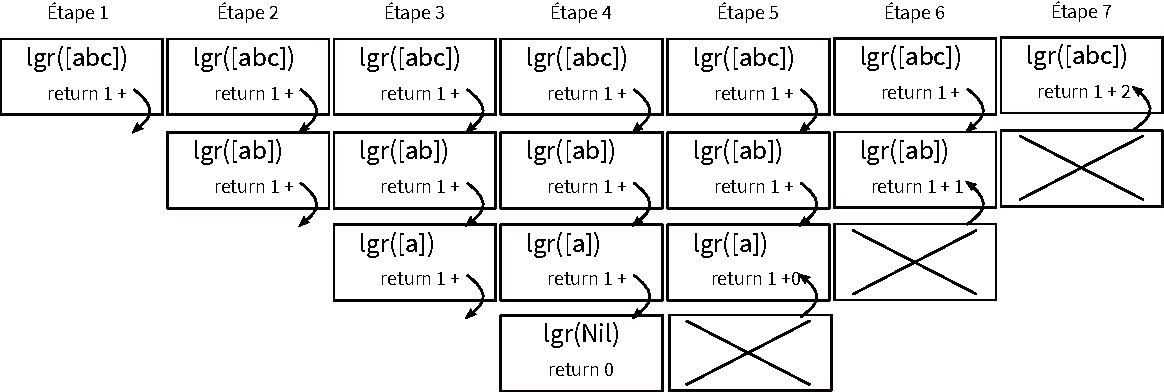
\includegraphics[width=\linewidth]{img/lgr.pdf}

      On retrouve bien la descente récursive et la remontée récursive vues en
      cours.

    \item[Terminaison:] La longueur est strictement décroissante et on s'arrête
      quand la chaîne est vide.
    \item[Correction:] On se contente de déplier les appels au tableau
      aujourd'hui. Mais il faut le faire pour qu'ils comprennent, et il faut le
      faire à chaque fois, pas que celui là.
    \item[Complexité:] On regarde chaque lettre, on a donc O(n) appels
      récursifs. A chaque appel, on n'appelle que des fonctions de base, pas
      chères. Donc une étape est en O(1). Résultat: $O(n)\times O(1)=O(n)$
  \end{description}

\medskip\noindent
\begin{minipage}{.48\linewidth}
  \begin{Verbatim}[label=écriture fonctionnelle (sans return)]
def length(l:List[Char]):Int = {
  if (l == Nil)
    0
  else 
    1 + length(l.tail)
}
  \end{Verbatim}  
\end{minipage}\hfill%
\begin{minipage}{.48\linewidth}
  \begin{Verbatim}[numbers=right,label=avec un zoli filtrage]
def length(l:List[Char]):Int = {
  l match {
    case a::b => 1 + length(b)
    case _    => 0
  }
}
  \end{Verbatim}  
\end{minipage}

\end{Reponse}

%%%%%%%% est_membre %%%%%%%%%%%%%%%%%%%%%%%%%%%%%%%%%%%%
\begin{Question}
  $est\_membre: \left\{
    \begin{array}{l}
      \Type{List[Char]}\times \Type{Char}\mapsto \Type{Boolean}\\
      \text{retourne \Type{true} ssi le caractère fait partie de la chaîne}
    \end{array}\right.$  
\end{Question}
\begin{Reponse}
\noindent
  \begin{minipage}{.43\linewidth}
  \begin{Verbatim}
def isMember(value:Char,
             l:List[Char]):Boolean= {
  if (l==Nil) false
  else if (l.head == value) true
  else isMember(value, l.tail)
}

  \end{Verbatim}    
  \end{minipage}
  \begin{minipage}{.55\linewidth}
  \begin{Verbatim}[numbers=right]
def isMember(v:Char, l:List[Char]):Boolean= {
  l match {
    case a::_ if a==v => true
    case a::b         => isMember(v, b)
    case _            => false
  }
}
  \end{Verbatim}        
  \end{minipage}

  \begin{description}
  \item[Est ce que cette fonction traite correctement le cas où le caractère
    n'est pas dedans.] ~\\ Appliquez le meme algo à la recherche d'une peau
    rouge dans un oignon. Je regarde la peau extérieure, elle est pas rouge, je
    l'enlève et recommence. Je recommence sur toutes les peaux (toutes jaunes)
    jusqu'à la toute dernière. Je l'enlève aussi car elle est jaune. Je me
    retrouve avec l'oignon vide entre les mains, j'ai donc l'assurance qu'aucune
    peau n'était rouge dans mon oignon.
  \item[Terminaison et Complexité:] comme avant. Simplement, chaine vide n'est
    pas le seul cas terminal, mais ca ne gène pas la terminaison. On pourrait
    chercher à faire une étude plus précise de la complexité avec meilleur des
    cas et pire des cas, mais ce n'est pas la peine. En moyenne, cet algo est
    linéaire. Faut juste leur faire sentir la complexité et laisser au module
    "Mat Num" le plaisir de faire des maths.
  \item[Complexité meilleur des cas] c'est si la chaine est vide ou qu'on
    cherche 't' dans 'toto'. $O(1)$
  \item[Complexité pire des cas] Je cherche 'e' dans 'toto', je dois parcourir
    toute la chaine. $O(n)$
  \item[Complexité cas moyen] Ben on peut pas répondre avec si peu de
    données. Ceux qui répondent [$\frac{n}{2}$] supposent l'équiprobabilité des
    lettres, c'est une hypothèse forte que l'on a pas. Imaginez chercher le ß
    (on le z) dans la langue française, par rapport au 'e'.
  \end{description}
\end{Reponse}

%%%%%%%% occurence %%%%%%%%%%%%%%%%%%%%%%%%%%%%%%%%%%%%
\begin{Question}
  $occurence: \left\{
    \begin{array}{l}
      \Type{Char}\times \Type{List[Char]}\mapsto \Type{Int}\\
      \text{retourne le nombre d'occurences du caractère dans la chaîne}
    \end{array}\right.$  
\end{Question}
\begin{Reponse}
  \begin{minipage}{.49\linewidth}
  \begin{Verbatim}
def occ(value:Char, l:List[Char]):Int= {
  if (l==Nil) 0
  else if (l.head == value) 
       1+occ(value, l.tail)
  else   occ(value, l.tail)
}

  \end{Verbatim}    
  \end{minipage}
  \begin{minipage}{.49\linewidth}
  \begin{Verbatim}[numbers=right]
def occ(v:Char, l:List[Char]):Int= {
  l match {
    case a::b if a==v => 1+occ(v, b)
    case a::b         =>   occ(v, b)
    case _            => 0
  }
}
  \end{Verbatim}        
  \end{minipage}
  \begin{description}
  \item[Terminaison et Complexité:] comme avant: $O(n)$. 
  \end{description}
\end{Reponse}

%%%%%%%% tous_differents %%%%%%%%%%%%%%%%%%%%%%%%%%%%%%%%%%%%
\begin{Question}
  $tous\_differents: \left\{
    \begin{array}{l}
      \Type{List[Char]}\mapsto \Type{Boolean}\\
      \text{retourne \Type{true} ssi tous les membres de la chaine sont différents}
    \end{array}\right.$  
\end{Question}
\begin{Reponse}
  \begin{Verbatim}[label=tous\_differents(ch)]
si ch = chvide alors VRAI
               sinon si est_membre(suite(ch), premier(ch)) alors FAUX
                                                     sinon tous_differents(suite(ch))    
  \end{Verbatim}
  \begin{Verbatim}
def allDifferent(l:List[Char]):Boolean = {
  if (l == Nil)                      true
  else if (isMember(l.head, l.tail)) false
  else                               allDifferent(l.tail)
}    
  \end{Verbatim}
  \begin{description}
  \item[Terminaison:] comme avant.
  \item[Complexité:] On fait toujours $O(n)$ appels récursifs, mais ce coup ci,
    chacun fait appel à est\_membre, qui est elle même en $O(n)$. Donc $C =
    O(n)\times O(n) = O(n^2)$

    On peut se poser la question de l'optimalité. Est ce que c'est comme ca que
    vous vérifiez que toutes les cartes d'un paquet sont différente ?? Non,
    bien sur. Le plus simple à la main, c'est de trier la pile dans un ordre
    donné, puis de faire un seul parcours en comparant chaque carte à la
    suivante (un peu comme la fonction croissante, donnée plus bas).

    Étant donné qu'il existe des algos de tris en $O(n\times log(n))$, on a
    $$C = C_{pretraitement}+C_{fonction recursive}= O(n\times log(n)) + O(n) =
    O(n\times log(n))$$ Ce qui est bien mieux que $O(n^2)$ quand n est grand.

    Notons cependant que la complexité dans le meilleur des cas passe de $O(1)$
    (quand la chaîne commence par 'aa', l'algo $O(n^2)$ répond immédiatement) à
    $O(n\times log(n)$... sauf si on a fait son tri avec attention.
  \end{description}
\end{Reponse}

%%%%%%%% supprime %%%%%%%%%%%%%%%%%%%%%%%%%%%%%%%%%%%%
\begin{Question}
  $supprime: \left\{
    \begin{array}{l}
      \Type{Char}\times\Type{List[Char]} \mapsto \Type{List[Char]}\\
      \text{retourne la chaine privée de toutes les occurences du caractère.}
    \end{array}\right.$  

  Si le caractère ne fait pas partie de la chaîne, celle-ci est inchangée.
\end{Question}
\begin{Reponse}
  \begin{Verbatim}
def remove(v:Char, l:List[Char]):List[Char]={
  l match {
    case a::b if a==v =>    remove(v, b)
    case a::b         => a::remove(v, b)
    case _            => Nil
  }
}    
  \end{Verbatim}
  \begin{description}
  \item[Terminaison et Complexité:] comme avant: $O(n)$. 
  \end{description}
\end{Reponse}

%%%%%%%% deuxieme %%%%%%%%%%%%%%%%%%%%%%%%%%%%%%%%%%%%
\begin{Question}
  $deuxieme: \left\{
    \begin{array}{l}
      \Type{List[Char]}\mapsto \Type{Char}\\
      \text{retourne le deuxième caractère de la chaîne}
    \end{array}\right.$  
\end{Question}
\begin{Reponse}
  \begin{Verbatim}[]
// PRECONDITION: list != Nil et ch.tail != Nil
def second(list: List[Char]):Char = list.tail.head
  \end{Verbatim}
  \begin{description}
  \item[Terminaison:] C'est un appel direct, sans récursion. Mais c'est
    l'occasion de parler des préconditions.  On ne vérifie pas explicitement si
    la précondition est respectée dans le code, car on ne saurait pas trop
    comment réagir si elle est violée. On laisse donc Scala se débrouiller, il
    va lever une exception comme il se doit. 

    Il faut bien insister sur cette histoire de précondition, c'est la raison
    d'être de cette question.

    Oui, au passage, les accolades sont optionnelles en Scala quand on défini
    une fonction.
  \item[Complexité:] O(1)
  \end{description}
\end{Reponse}

%%%%%%%% dernier %%%%%%%%%%%%%%%%%%%%%%%%%%%%%%%%%%%%
\begin{Question}
  $dernier: \left\{
    \begin{array}{l}
      \Type{List[Char]}\mapsto \Type{Char}\\
      \text{retourne le dernier caractère de la chaîne}
    \end{array}\right.$  
\end{Question}
\begin{Reponse}
  \begin{Verbatim}[]
// PRECONDITION: list != Nil
def last(list:List[Char]): Char = {
  if (list.tail == Nil) list.head
  else                  last(list.tail)
}
  \end{Verbatim}
  \begin{description}
  \item[Terminaison et Complexité:] comme avant: $O(n)$. 
  \end{description}
\end{Reponse}

%%%%%%%% saufdernier %%%%%%%%%%%%%%%%%%%%%%%%%%%%%%%%%%%%
\begin{Question}
  $saufdernier: \left\{
    \begin{array}{l}
      \Type{List[Char]}\mapsto \Type{List[Char]}\\
      \text{retourne la chaine privée de son dernier caractère}
    \end{array}\right.$  
\end{Question}
\begin{Reponse}
  \begin{Verbatim}
// PRECONDITION: list != Nil
def butLast(list: List[Char]): List[Char] = {
  if (list.tail == Nil) Nil
  else                  list.head :: butLast(list.tail)
}
  \end{Verbatim}
  \begin{description}
  \item[Terminaison et Complexité:] comme avant: $O(n)$. 
  \end{description}
\end{Reponse}

%%%%%%%% nieme %%%%%%%%%%%%%%%%%%%%%%%%%%%%%%%%%%%%
\begin{Question}
  $nieme: \left\{
    \begin{array}{l}
      \Type{List[Char]}\times\Type{Int}\mapsto \Type{Char}\\
      \text{retourne le nieme caractère de la chaîne}
    \end{array}\right.$  
\end{Question}
\begin{Reponse}
  \begin{Verbatim}
// PRECONDITION: list != Nil
def nth(list: List[Char], rank: Int): Char = {
  if (rank==0) list.head
  else         nth(l.tail, rank-1)
}
  \end{Verbatim}
  \begin{description}
  \item[Terminaison et Complexité:] comme avant: $O(n)$. 
  \end{description}
\end{Reponse}

%%%%%%%% npremiers %%%%%%%%%%%%%%%%%%%%%%%%%%%%%%%%%%%%
\begin{Question}
  $npremiers: \left\{
    \begin{array}{l}
      \Type{List[Char]}\times\Type{Int}\mapsto \Type{List[Char]}\\
      \text{retourne les n premiers caractères de la chaîne}
    \end{array}\right.$  
\end{Question}
\begin{Reponse}
  \begin{Verbatim}
// PRECONDITION: n>=list.size
def nFirsts(list: List[Char], amount:Int):List[Char] = {
  if (amount == 0) Nil
  else             l.head :: nFirsts(l.tail, amount-1)
}
  \end{Verbatim}
  \begin{description}
  \item[Terminaison et Complexité:] comme avant: $O(n)$.
  \item[Correction:] C'est un bon exemple pour faire une preuve de correction:
    \begin{itemize}
    \item Précondition à l'étape $n$ entraine (récursivement) la précondition
      pour les étapes suivantes avec des $n$ plus petits
    \item Le traitement dans le cas terminal (pour $n=0$) assure la
      post-condition
    \item Le traitement lors de la remontée assure la post-condition
    \end{itemize}
  \end{description}
\end{Reponse}

%%%%%%%% nderniers %%%%%%%%%%%%%%%%%%%%%%%%%%%%%%%%%%%%
\begin{Question}
  $nderniers: \left\{
    \begin{array}{l}
      \Type{List[Char]}\times\Type{Int}\mapsto \Type{List[Char]}\\
      \text{retourne les n derniers caractères de la chaîne}
    \end{array}\right.$  
\end{Question}
\begin{Reponse}
  Plusieurs variantes sont possibles:
  \begin{Verbatim}[label=version naive]
def nLasts(list: List[Char], amount:Int):List[Char] = {
  if (amount==list.size) list
  else nLasts(list.tail, n-1)
}    
  \end{Verbatim}
  \begin{description}
  \item[Complexité:] On a $O(n)$ appels récurssifs, mais chacun fait un appel à
    longueur, qui est elle même en $O(n)$. Donc, $C=0(n)\times
    O(n)=O(n^2)$. 
  \end{description}

  \begin{Verbatim}[label=avec retourne]
def nLasts(l:List[Char], n:Int):List[Char] = reverse(nFirst(reverse(list),n))
  \end{Verbatim}
  \begin{description}
  \item[Complexité:] On ajoute les complexités respectives de chaque appel. $C =
    O(n) + O(n) + O(n) = O(n)$, (car $C_{retourne}=O(n)$) ce qui est mieux. Mais
    retourne n'est pas encore défini, ce qui donne l'impression de tricher un
    peu. Alors on fait une troisième version, qui est surtout l'occasion
    d'introduire les fonctions helpers.
  \end{description}

  \begin{Verbatim}[label=avec fonction d'aide]
def nLasts(list:List[Char], n:Int):List[Char] = {
  butNFirsts(list, list.size-n) 

  def butNFirst(list:List[Char], n:Int):List[Char] = {
    if (n==0 || list==Nil) list
    else      butNFirst(list.tail, n-1)
  }
}
  \end{Verbatim}

  L'idée est donc de calculer une bonne fois pour toute combien de caractères
  il faut retirer, puis de le faire ensuite sans réflechir au lieu de (comme
  dans la première) regarder apres chaque retrait si on en a enlevé assez. Ca
  permet de tomber la complexité en $O(n)$.
\end{Reponse}

%%%%%%%% retourne %%%%%%%%%%%%%%%%%%%%%%%%%%%%%%%%%%%%
\begin{Question}
  $retourne: \left\{
    \begin{array}{l}
      \Type{List[Char]}\mapsto \Type{List[Char]}\\
      \text{retourne la chaine lue en sens inverse}
    \end{array}\right.$  
\end{Question}
\begin{Reponse}
  Cette fonction est très importante. Si vous manquez de temps, faites sauter
  d'autres fonction pour parvenir à faire celle là car on en a très besoin dans
  le TP2. Là encore, il y a plusieurs solutions.
  \begin{Verbatim}[label=version bourinne]
def reverse(l:List[Char]):List[Char]={
  if (l == Nil) Nil
  else          last(l) :: reverse(butLast(l))
}
  \end{Verbatim}
  \begin{description}
  \item[Complexité:] $O(n)$ appels, et $O(n)$ chaque à cause de saufdernier et
    dernier. $O(n^2)$, donc.
  \end{description}
  
  \textbf{Comment leur faire trouver mieux:} Demandez leur de réfléchir à
  comment ils inversent l'ordre d'une pile de cartes, ou une pile d'assiettes: on prend une pile 
  supplémentaire, on passe le premier de la pile de départ sur l'autre, et on
  recommence avec la deuxieme de la pile de départ. Si ca aide pas, faut
  détailler un exemple:
  A trier ABC $\leadsto$ \begin{tabular}{|l l|}\hline
    ABC&$\emptyset$\\
    BC&A\\
    C&BA\\
    $\emptyset$&CBA\\\hline
  \end{tabular}$\leadsto$ résulat = CBA

  \begin{Verbatim}[label=avec helper]
def retourne(l:List[Char]):List[Char] = {

  def helper(todo:List[Char], done:List[Char]): List[Char] = {
    if (todo==Nil) done
    else           helper(todo.tail, todo.head :: done )
  }

  helper(l, Nil)
}
  \end{Verbatim}
  Comme souvent avec les fonctions helpers, on construit dans un argument
  supplémentaire le résultat final. Donc, on prend le travail qu'on aurait fait
  pendant la remontée, et on le fait dans la descente sur cet
  accumulateur. C'est important car ça change la fonction en récursive
  terminale (même s'ils n'ont pas encore vu ce que c'est à ce moment du cours).

  Ce qui nous interresse ici, c'est que la complexité passe en $O(n)$. Il est
  très important de déplier le retournement d'une chaîne d'exemple avec cette
  méthode. 

\end{Reponse}

%%%%%%%% concat %%%%%%%%%%%%%%%%%%%%%%%%%%%%%%%%%%%%
\begin{Question}
  $concat: \left\{
    \begin{array}{l}
      \Type{List[Char]}\times \Type{List[Char]}\mapsto \Type{List[Char]}\\
      \text{retourne les deux chaines concaténées}
    \end{array}\right.$  
\end{Question}
\begin{Reponse}
  \begin{Verbatim}[label=version brutale: $O(n^2)$]
def concat1(ch1:List[Char], ch2:List[Char]): List[Char] = {
  if (ch1 == Nil) return ch2
  return concat1(butLast(l), last(ch1)::ch2)
}
  \end{Verbatim}

  Pour aller plus vite, il faut mettre ch1 à l'envers une bonne fois pour toute
  au lieu d'aller piocher le dernier à tout bout de champ. On passe de
  $O(n^2)$ à $O(n)$, tout de même. Encore une fois, un exemple donné avant les
  aide à trouver tous seuls.
  \medskip

  \begin{tabular}{|l l l|}\hline
    ABC&DEF& en donnée\\
    CBA&DEF& on inverse ch1 avant d'appeller helper\\
    BA&CDEF& récursion dans helper\\
    A&BCDEF& récursion dans helper\\
    $\emptyset$&ABCFED& Cas terminal de la récursion dans helper\\\hline
  \end{tabular}$\leadsto$ résultat = ABCDEF

  \begin{Verbatim}[label=version avec helper: $O(n)$]
def concat(ch1:List[Char], ch2:List[Char]):List[Char] = {
  def helper(ch1:List[Char], ch2:List[Char]):List[Char] = {
    if (ch1 == Nil) return ch2
    else return helper(ch1.tail, ch1.head :: ch2)
  }
  helper(reverse(ch1), ch2)
}
  \end{Verbatim}
  
  On peut même se rendre compte que notre helper est exactement le
  même que celui de reverse. Du coup, on peut réécrire ainsi:
  
  \begin{Verbatim}[label=version avec helper: $O(n)$]
def concat(ch1:List[Char], ch2:List[Char]):List[Char] = {
  def helper(ch1:List[Char], ch2:List[Char]):List[Char] = {
    if (ch1 == Nil) return ch2
    else return helper(ch1.tail, ch1.head :: ch2)
  }
  helper( helper(ch1, Nil), ch2)
}
  \end{Verbatim}
\end{Reponse}

%%%%%%%% min_ch %%%%%%%%%%%%%%%%%%%%%%%%%%%%%%%%%%%%
\begin{Question}
  $min\_ch: \left\{
    \begin{array}{l}
      \Type{List[Char]}\mapsto \Type{Char}\\
      \text{retourne le caractère le plus petit de la chaîne}
    \end{array}\right.$  
  
  \smallskip
  On considère l'ordre lexicographique, et on suppose l'existance d'une
  fonction min(a,b).
\end{Question}
\begin{Reponse}
  \begin{Verbatim}[label=min\_ch(ch)]
PRECONDITION: ch != chvide
def min(l:List[Char]): Char = {
  def min2(l:List[Char], v:Char): Char = {
    if (l==Nil) return v
    if (l.head < v) return min2(l.tail, l.head)
    return min2(l.tail, v)
  }
  return min2(l.tail, l.head)
}
  \end{Verbatim}

  \begin{description}
  \item[Terminaison et Complexité:] comme avant: $O(n)$. 
  \end{description}
\end{Reponse}

%%%%%%%% croissante %%%%%%%%%%%%%%%%%%%%%%%%%%%%%%%%%%%%
\begin{Question}
  $croissante: \left\{
    \begin{array}{l}
      \Type{List[Char]}\mapsto bool\acute{e}en\\
      \text{retourne si la chaine est croissante (dans l'ordre lexicographique)}
    \end{array}\right.$  
\end{Question}
\begin{Reponse}
  \begin{Verbatim}[label=croissante(ch)]
def increasing(l:List[Int]): Boolean = {
  if (l == Nil || l.tail == Nil) return true
  if (l.head > l.tail.head)      return false
  return increasing(l.tail)
}
  \end{Verbatim}
  \begin{description}
  \item[Terminaison et Complexité:] comme avant: $O(n)$. 
  \end{description}
\end{Reponse}

%%%%%%%% nnaturels %%%%%%%%%%%%%%%%%%%%%%%%%%%%%%%%%%%%
\begin{Question}
  $nnaturels: \left\{
    \begin{array}{l}
      \Type{Int}\mapsto \Type{List[Int]}\\
      \text{retourne une chaine formée des n premiers entiers naturels}
    \end{array}\right.$  
  
  Dans un premier temps, on construira $\{n, n-1, n-2, \ldots, 3, 2, 1\}$ avant
  de construire $\{1, 2, 3, \ldots, n\}$.
\end{Question}
\begin{Reponse}
  \begin{Verbatim}[label=Version simple qui donne la liste à l'envers]
nnaturels1(n):
  si n = 0 alors chvide
           sinon adj(n, nnaturels1(n-1))
  \end{Verbatim}

  \begin{Verbatim}[label=Version trichée qui donne la chaine à l'endroit:]
nnaturels2(n):
  retourne(nnaturels1(ch))
  \end{Verbatim}
  
  Pour faire la série dans l'ordre sans tricher, il faut une fonction
  d'aide. Pour le faire trouver, on peut écrire au tableau les différents
  arguments pris par cette fonction d'aide.
  \begin{Verbatim}[label=Version avec helper:]
nnaturels3(n):
  nnaturels3_helper(1,n-1)    

nnaturels3_helper(n, todo):
  si todo = 0 alors chvide
              sinon adj(n, nnaturels3_helper(n+1,todo-1)
  \end{Verbatim}
\end{Reponse}


%%%%%%%% palindrome %%%%%%%%%%%%%%%%%%%%%%%%%%%%%%%%%%%%
\begin{Question}
  $palindrome: \left\{
    \begin{array}{l}
      \Type{List[Char]}\mapsto bool\acute{e}en\\
      \text{retourne VRAI si la chaine est un palindrome}
    \end{array}\right.$  

  Un palindrome se lit indifféremment de droite à gauche ou de gauche à droite.
  Exemple : « Esope reste et se repose ». On peut ignorer les espaces.
\end{Question}
\begin{Reponse}
  \begin{Verbatim}[label=palindrome(ch)]
si longueur(ch) <= 1 alors 
  VRAI
sinon
  si premier(ch) = dernier(ch) alors
    palindrome(suite(saufdernier(ch)))
  sinon 
    si premier(ch) = ' ' alors
      palindrome(suite(ch))
    sinon 
      si dernier(ch) = ' ' alors
        palindrome(saufdernier(ch))
      sinon
        FAUX
      finsi
    finsi    
  finsi
finsi    
  \end{Verbatim}
  La version simple est de ne pas ignorer les espaces, et de
  mettre un FAUX après le second «sinon» sans tester plus en avant.
\end{Reponse}

%%%%%%%% anagramme %%%%%%%%%%%%%%%%%%%%%%%%%%%%%%%%%%%%
\begin{Question}
  $anagramme: \left\{
    \begin{array}{l}
      \Type{List[Char]}\times \Type{List[Char]}\mapsto bool\acute{e}en\\
      \text{retourne VRAI si les chaines sont des anagrammes l'une de l'autre}
    \end{array}\right.$  

  Une anagramme d'un mot est un autre mot obtenu en permutant les lettres.
  Exemples: «chien» et «niche»; «baignade» et «badinage»; «Séduction»,
  «éconduits» et «on discute».
\end{Question}
\begin{Reponse}
  \begin{Verbatim}[label=anagramme(ch1\quotesinglbase ch2)]
si ch1=chvide et ch2=chvide alors
  VRAI
sinon
  si est_membre(premier(ch1), ch2) alors
    anagramme(suivant(ch1), supprime(premier(ch1), ch2))
  sinon
    FAUX
  finsi
finsi
  \end{Verbatim}
\end{Reponse}

%%%%%%%% union %%%%%%%%%%%%%%%%%%%%%%%%%%%%%%%%%%%%
\begin{Question}
  $union: \left\{
    \begin{array}{l}
      \Type{List[Char]}\times \Type{List[Char]}\mapsto \Type{List[Char]}\\
      \text{retourne une chaîne formée de toutes les lettres de ch1 et ch2,
        sans doublons}
    \end{array}\right.$    
  On peut supposer dans un premier temps que ch1 et ch2 ne contiennent pas de
  doublons.
\end{Question}
\begin{Reponse}
  \begin{Verbatim}[label=union(ch1\quotesinglbase ch2)]
si ch1=chvide alors
  si ch2=chvide alors
    chvide
  sinon
    union(ch2,chvide) -- Pour virer les doublons de ch2
  finsi
sinon
  si est_membre(premier(ch1), suite(ch1)) ou est_membre(premier(ch1), ch2) alors
    union(suite(ch1),ch2)
  sinon
    adj(premier(ch1),union(suite(ch1),ch2))
  finsi
finsi    
  \end{Verbatim}
\end{Reponse}

%%%%%%%% difference %%%%%%%%%%%%%%%%%%%%%%%%%%%%%%%%%%%%
\begin{Question}
  $difference: \left\{
    \begin{array}{l}
      \Type{List[Char]}\times \Type{List[Char]}\mapsto \Type{List[Char]}\\
      \text{retourne toutes les lettres de ch1 ne faisant
        pas partie de ch2}
    \end{array}\right.$    
\end{Question}
\begin{Reponse}
  \begin{Verbatim}[label=difference(ch1\quotesinglbase ch2)]
si ch2 = chvide alors
  ch1
sinon 
  si ch1 = chvide alors
    chvide
  sinon
    si est_membre(premier(ch1),ch2) alors
      difference(suite(ch1),ch2)
    sinon
      adj(premier(ch1), difference(suite(ch1),ch2))
    finsi
  finsi
finsi    
  \end{Verbatim}
\end{Reponse}

\end{document}
%%% Local Variables:
%%% coding: utf-8
